% Options for packages loaded elsewhere
\PassOptionsToPackage{unicode}{hyperref}
\PassOptionsToPackage{hyphens}{url}
\PassOptionsToPackage{dvipsnames,svgnames,x11names}{xcolor}
%
\documentclass[
  10pt,
]{article}
\usepackage{amsmath,amssymb}
\usepackage{iftex}
\ifPDFTeX
  \usepackage[T1]{fontenc}
  \usepackage[utf8]{inputenc}
  \usepackage{textcomp} % provide euro and other symbols
\else % if luatex or xetex
  \usepackage{unicode-math} % this also loads fontspec
  \defaultfontfeatures{Scale=MatchLowercase}
  \defaultfontfeatures[\rmfamily]{Ligatures=TeX,Scale=1}
\fi
\usepackage{lmodern}
\ifPDFTeX\else
  % xetex/luatex font selection
\fi
% Use upquote if available, for straight quotes in verbatim environments
\IfFileExists{upquote.sty}{\usepackage{upquote}}{}
\IfFileExists{microtype.sty}{% use microtype if available
  \usepackage[]{microtype}
  \UseMicrotypeSet[protrusion]{basicmath} % disable protrusion for tt fonts
}{}
\makeatletter
\@ifundefined{KOMAClassName}{% if non-KOMA class
  \IfFileExists{parskip.sty}{%
    \usepackage{parskip}
  }{% else
    \setlength{\parindent}{0pt}
    \setlength{\parskip}{6pt plus 2pt minus 1pt}}
}{% if KOMA class
  \KOMAoptions{parskip=half}}
\makeatother
\usepackage{xcolor}
\usepackage[margin=0.85in]{geometry}
\usepackage{longtable,booktabs,array}
\usepackage{calc} % for calculating minipage widths
% Correct order of tables after \paragraph or \subparagraph
\usepackage{etoolbox}
\makeatletter
\patchcmd\longtable{\par}{\if@noskipsec\mbox{}\fi\par}{}{}
\makeatother
% Allow footnotes in longtable head/foot
\IfFileExists{footnotehyper.sty}{\usepackage{footnotehyper}}{\usepackage{footnote}}
\makesavenoteenv{longtable}
\usepackage{graphicx}
\makeatletter
\def\maxwidth{\ifdim\Gin@nat@width>\linewidth\linewidth\else\Gin@nat@width\fi}
\def\maxheight{\ifdim\Gin@nat@height>\textheight\textheight\else\Gin@nat@height\fi}
\makeatother
% Scale images if necessary, so that they will not overflow the page
% margins by default, and it is still possible to overwrite the defaults
% using explicit options in \includegraphics[width, height, ...]{}
\setkeys{Gin}{width=\maxwidth,height=\maxheight,keepaspectratio}
% Set default figure placement to htbp
\makeatletter
\def\fps@figure{htbp}
\makeatother
\setlength{\emergencystretch}{3em} % prevent overfull lines
\providecommand{\tightlist}{%
  \setlength{\itemsep}{0pt}\setlength{\parskip}{0pt}}
\setcounter{secnumdepth}{5}
\usepackage{float}
\floatplacement{figure}{H}
\ifLuaTeX
  \usepackage{selnolig}  % disable illegal ligatures
\fi
\IfFileExists{bookmark.sty}{\usepackage{bookmark}}{\usepackage{hyperref}}
\IfFileExists{xurl.sty}{\usepackage{xurl}}{} % add URL line breaks if available
\urlstyle{same}
\hypersetup{
  pdftitle={When Does Hamiltonian Structure Help Control?},
  pdfauthor={Jiajun Fu (Duke Kunshan University)},
  colorlinks=true,
  linkcolor={blue},
  filecolor={Maroon},
  citecolor={Blue},
  urlcolor={blue},
  pdfcreator={LaTeX via pandoc}}

\title{When Does Hamiltonian Structure Help Control?}
\usepackage{etoolbox}
\makeatletter
\providecommand{\subtitle}[1]{% add subtitle to \maketitle
  \apptocmd{\@title}{\par {\large #1 \par}}{}{}
}
\makeatother
\subtitle{A reproducible study of coverage, coordinate priors, model
error and policy optimization}
\author{Jiajun Fu (Duke Kunshan University)}
\date{October 2026}

\begin{document}
\maketitle

\hypertarget{abstract}{%
\section*{Abstract}\label{abstract}}
\addcontentsline{toc}{section}{Abstract}

Hamiltonian structure is a useful inductive bias, but its contribution
to downstream control can be obscured by known mechanics, coordinates,
data coverage and policy optimization. We present a reproducible study
that separates these factors using controlled pendulum systems, exact
Fourier force regressors, neural world models, finite-budget soft
actor-critic (SAC), fixed feedback and model predictive control. The
central contribution is an experimental decomposition of apparent
structure advantages, with independently checked mathematical
diagnostics and a retained negative acquisition result. In a
validation-selected coupled-pendulum benchmark, Hamiltonian force
estimation improves local extrapolation, while global coverage
substantially narrows the gap. An incorrectly centered parity prior has
an explicit approximation floor, removed by privileged recentering.
Independent coupled Duffing validation reproduces the dominant coverage
effect. A frozen task-weighted acquisition candidate fails all four
primary tracking cells despite reducing its posterior uncertainty
criterion. Finally, exact-force control exhibits first-order action-hold
error, separating a numerical controller floor from model uncertainty.
These findings support conditional, task-specific interpretations of
structure rather than a universal Hamiltonian advantage. The study
supplies original computational results and a self-contained analytical
synthesis; it does not introduce a new general learning algorithm or
assert novelty of classical regression, filtering or invariant-design
results.

\textbf{Keywords:} Hamiltonian learning; model-based reinforcement
learning; experimental design; data coverage; coordinate priors; sampled
control.

\hypertarget{introduction}{%
\section{Introduction}\label{introduction}}

A dynamics model can conserve its own learned energy and still predict
the wrong physical trajectory. A more accurate dynamics model can also
fail to improve a learned policy when optimization is the limiting
factor. Both distinctions matter when Hamiltonian world models are used
for reinforcement learning.

Our question is: \textbf{when does Hamiltonian structure improve
cross-energy prediction and control after accounting for coordinate
representations, mechanical priors, coverage, regularization and
optimization?} We investigate the question through staged, paired
interventions. The initial single-pendulum experiments motivate the
stronger multidimensional comparisons, rather than supply a stand-alone
claim of algorithmic superiority. The main analysis uses
finite-dimensional force spaces whose regression objectives can be
solved and verified directly. This makes it possible to distinguish
model fitting from policy optimization.

The study contributes three linked pieces of original experimental
evidence. First, a coverage and coordinate-origin benchmark compares
equal-dimensional parity and Hamiltonian subspaces, supplemented by a
correctly recentered parity diagnostic. Second, a predeclared
acquisition screen demonstrates a gap between a task-weighted covariance
objective and actual held-action tracking. Third, an independent
quartic-system validation and action-hold refinement check test the main
alternative explanations. Classical mathematical identities connect
these experiments; they are attributed as background rather than
promoted as new theorems.

This is an original research manuscript reporting newly executed
simulations and analyses. It is not a certificate that no similar
empirical observation has appeared previously, and it is not a claim
that the failed candidate is a novel successful algorithm. The
manuscript is suitable as a reproducible research report and a basis for
scholarly review. Submission, venue fit and acceptance require
independent assessment.

\hypertarget{related-work-and-scope-of-originality}{%
\section{Related work and scope of
originality}\label{related-work-and-scope-of-originality}}

Hamiltonian neural networks parameterize a scalar energy and obtain the
vector field through canonical differentiation {[}1{]}. Controlled
Hamiltonian learning has also been developed in Symplectic ODE-Net
{[}2{]}. These works motivate the structural model families; our convex
feature experiments do not replicate their full architectures.

Gruver et al.~already analyze second-order modeling and coordinate
complexity as explanations of Hamiltonian-network performance {[}3{]}.
Accordingly, deconstructing physical priors is not a new general agenda.
Our contribution is the particular coverage intervention,
coordinate-origin comparison, controlled optimization separation and
unsuccessful acquisition record, together with independently
reproducible diagnostics. Claims about the source of performance are
confined to the systems and model classes tested here.

Hamiltonian and odd-symmetry kernel/random-feature models are
established approaches {[}4{]}. Our Fourier heads are transparent
finite-dimensional comparators, not exact implementations of that
published kernel algorithm. Task-optimal exploration in linear and
nonlinear dynamics already uses task-dependent estimation metrics
{[}5,6{]}. Bayesian active reinforcement learning {[}7{]} and
transition-occupancy matching {[}8{]} address additional policy-relevant
information. The spectral acquisition used here specializes weighted
experimental design to periodic tracking; neither its weighted trace nor
Gaussian covariance update is new. We do not compare against full
implementations of those algorithms and cannot claim to outperform them.

Invariant-design symmetrization is classical {[}9,10{]}. The torus
specialization below explains why frequency weighting alone need not
favor nonuniform query locations. It is explanatory analysis added after
the frozen gate, with assumptions that intentionally exclude the actual
fixed local pilot.

\hypertarget{systems-representations-and-information-access}{%
\section{Systems, representations and information
access}\label{systems-representations-and-information-access}}

\hypertarget{controlled-mechanics}{%
\subsection{Controlled mechanics}\label{controlled-mechanics}}

We study separable systems with known unit kinetic energy and torque
ports,

\[H(q,p)=\frac12\|p\|^2+V(q),\qquad \dot q=p,\quad \dot p=F(q)+u,\quad F=-\nabla V.\]

Every multidimensional comparator knows these kinematics and input
channels. Thus the measured structural effect concerns the force
representation, not discovery of unknown inertia or canonical
coordinates. With control, the true energy balance is
\(\dot H=p^\top u\). Energy diagnostics use signed work and do not imply
energy conservation during actuation.

The periodic potential is

\[\begin{aligned}
V_s(q)={}&1-\cos(q_1-s_1)+0.8[1-\cos(q_2-s_2)]\\
&+0.3[1-\cos(q_1-q_2-s_1+s_2)]\\
&+\varepsilon[1-\cos(3(q_1-s_1)-(q_2-s_2))].
\end{aligned}\]

Canonical, misspecified and shifted conditions use
\((\varepsilon,s)=(0,0)\), \((0.06,0)\) and \((0.06,(0.45,-0.35))\). The
shifted condition is a coordinate-origin probe of the same physics, not
independent physical replication.

The independent validation uses a coupled Duffing potential on
\(\mathbb R^2\),

\[V_D(x,y)=0.5x^2+0.65y^2+0.1(x-y)^2+0.25x^4+0.2y^4.\]

This changes domain and functional family; its validation concerns force
estimation only. No Duffing SAC or control-transfer result is claimed.

\hypertarget{force-spaces}{%
\subsection{Force spaces}\label{force-spaces}}

The periodic force expansion uses twelve representatives,

\[\mathcal K=\{(a,b):a=1,2,\ b=-2,\ldots,2\}\cup\{(0,1),(0,2)\},\]

\[F(q)=c+\sum_{k\in\mathcal K}[A_k\cos(k^\top q)+B_k\sin(k^\top q)].\]

Unrestricted force has 50 coefficients. Odd force sets \(c=A_k=0\) and
has 24. Hamiltonian force has zero mean and coefficients parallel to
\(k\), also with 24. Odd Hamiltonian force has 12. Equal parameter count
removes one confound; it does not make the two 24-dimensional spaces
identical in geometry or expressivity. Soft mean/curl penalties retain
50 coefficients, with statistical effective degrees of freedom depending
on regularization.

The Duffing comparison uses all force monomials of degree at most three
(20 coefficients), odd-degree force monomials (12), or gradients of
nonconstant potentials of degree at most four (14). Dimensions are
explicitly different. No Duffing result is presented as a
parameter-matched structure comparison.

\hypertarget{budgets-and-split-discipline}{%
\subsection{Budgets and split
discipline}\label{budgets-and-split-discipline}}

The main coverage experiment uses 4,096 training and 1,024 independent
validation force pairs per condition, three world seeds and local/global
coverage fractions 0, approximately 0.1 and 1. Sample counts are fixed.
Ridge and soft penalties are chosen by validation force error before
fresh test evaluation. There are 162 selected models from 1,620
candidates. Selection is not based on policy return.

The final diagnostic protocol is separately frozen before its outcomes,
after the earlier results are known. It uses five fresh seeds, 512
Duffing labels per coverage condition, noise standard deviation 0.03 and
fixed ridge \(10^{-6}\). Local configurations lie in \([-0.35,0.35]^2\)
and global/test configurations in \([-1.5,1.5]^2\). A shared 4,096-point
test estimates global force RMS. Prefix replacement and shared noise
pair coverage conditions. This diagnostic tests a specified explanation
rather than supplies an independent preregistration of the whole study.

Generative force queries are synthetic. Reachability, sensor cost,
contacts and unknown input dynamics are not modeled. Zero additional
truth queries during model-only policy training must not be confused
with zero world-model pretraining labels.

\hypertarget{analytical-decomposition}{%
\section{Analytical decomposition}\label{analytical-decomposition}}

\hypertarget{learned-energy-and-identifiable-physics}{%
\subsection{Learned energy and identifiable
physics}\label{learned-energy-and-identifiable-physics}}

Antisymmetry gives \(\nabla\widehat H^\top J\nabla\widehat H=0\): exact
Hamiltonian flow conserves its own energy. This places no quantitative
bound on conservation of the true \(H\) without a relation between \(H\)
and \(\widehat H\). A smooth potential perturbation supported outside
observed configurations can leave all local force labels unchanged and
alter unseen dynamics. Structural consistency therefore does not
identify the unobserved potential. These are classical facts,
illustrated here by explicit work and missing-mode experiments.

On a torus, curl-free force additionally requires zero cycle periods to
be a gradient of a periodic potential. A constant force bias has zero
curl but nonzero cycle work. Our earlier exact-error intervention holds
global force RMS at 0.04 across three error types: conservative
perturbations produce bounded true-energy error in the stated
construction, while a constant bias produces substantial secular work.
This is an analytic intervention, not evidence that learned models
necessarily exhibit those exact errors.

\hypertarget{coordinates-and-approximation-floors}{%
\subsection{Coordinates and approximation
floors}\label{coordinates-and-approximation-floors}}

Translation rotates each sine/cosine coefficient pair. Full Fourier and
Hamiltonian spaces are translation-closed; sine-only odd spaces
generally are not. The omitted harmonic \(k_*=(3,-1)\) gives the exact
squared force approximation floor

\[\inf_{\widehat F}\|\widehat F-F\|_{L^2(\mathbb T^2)}^2=\frac{\varepsilon^2\|k_*\|^2}{2}=5\varepsilon^2.\]

For \(\varepsilon=0.06\), the RMS floor is 0.134164. Oddness about an
incorrect origin adds

\[\frac12\sum_{j\in\{1,2,d\}}a_j^2\|k_j\|^2\sin^2(k_j^\top s)\]

to that squared floor, giving approximately 0.4435 for the stated shift.
Known-center recentering removes the added parity term. It does not
identify an unknown symmetry center for free and does not remove the
missing mode.

\hypertarget{conditional-estimation-variance}{%
\subsection{Conditional estimation
variance}\label{conditional-estimation-variance}}

Let \(v=T\theta\) encode a structural subspace, \(D\) the empirical
feature Gram matrix and \(R\) the population force-norm metric. For a
fixed design and fixed quadratic regularizer, write
\(A_T=T^\top(D+\lambda R+Q)T\). Independent componentwise noise variance
\(\sigma^2\) gives

\[\operatorname{Cov}(\widehat\theta\mid q)=\frac{\sigma^2}{N}A_T^{-1}D_TA_T^{-1},\qquad D_T=T^\top DT,\]

\[\mathcal V=\frac{\sigma^2}{N}\operatorname{tr}(R_TA_T^{-1}D_TA_T^{-1}).\]

After population whitening without soft penalties, this becomes

\[\mathcal V=\frac{\sigma^2}{N}\sum_j\frac{d_j}{(d_j+\lambda)^2}.\]

Local coverage can create small design eigenvalues and large noise
amplification. A valid restricted subspace changes both dimension and
restricted spectrum; broad coverage raises poorly observed directions.
This is a variance identity, not total risk, a bound on extrapolation
bias or the unconditional risk of validation-selected ridge. A separate
2,000-perturbation audit verifies the fixed-ridge calculation without
changing selected models.

\hypertarget{periodic-tracking-and-acquisition}{%
\subsection{Periodic tracking and
acquisition}\label{periodic-tracking-and-acquisition}}

For continuous unsaturated feedback \(u=-F_0(q)-\kappa(p-p_*)\), a small
force perturbation \(\delta F\) induces first-order error

\[\dot e_1+\kappa e_1=\delta F(q_0+p_*t).\]

For mode frequency \(\omega_k=k^\top p_*\), uniform-phase steady
response has squared contribution

\[\frac{\|A_k\|^2+\|B_k\|^2}{2(\kappa^2+\omega_k^2)}.\]

This is a standard stable-filter calculation, local in perturbation
amplitude and time. It is not a guarantee for actuator saturation,
finite-horizon phase drift, full policy return or optimal RL.

Force-whitened features \(B(q)\) use scalar prior precision
\(\rho=0.05\) and noise variance \(\sigma^2\). With
\(A=\rho I+\sum B_i^\top B_i\), posterior covariance is
\(\Sigma=\sigma^2A^{-1}\). Task design minimizes
\(\operatorname{tr}(W\Sigma)\); Woodbury gives the exact rank-two
covariance gain. This covariance excludes misspecification bias.

\textbf{Proposition (classical invariant-design specialization).}
Suppose the force space is translation-closed, \(W\) commutes with its
orthogonal translation representation, and the only fixed information is
scalar \(\rho I\). For approximate design \(\xi\),
\(M(\xi)=\int B^\top B\,d\xi\), Haar-uniform design minimizes
\(\operatorname{tr}[W(\rho I+nM)^{-1}]\).

\textbf{Proof.} Translation maps \(M\) to \(O_s^\top M O_s\) without
changing the criterion. Haar-averaging the translated design gives
uniform configuration measure and, by force whitening, information
\(I\). Convexity of inverse weighted trace and Jensen's inequality yield
\(\Psi(I)\le\int\Psi(O_s^\top MO_s)\,ds=\Psi(M)\). This establishes
optimality, not uniqueness. The actual nonuniform pilot violates the
assumption; finite random sampling is not identical to approximate
uniform design. The sine-only class also lacks translation closure.
\(\square\)

\hypertarget{sample-and-hold-error-with-an-exact-force-model}{%
\subsection{Sample-and-hold error with an exact force
model}\label{sample-and-hold-error-with-an-exact-force-model}}

A true-force controller can have nonzero error because actions are held.
The following consistency statement specializes ordinary sampled-control
analysis, rather than proposing a new control theorem.

\textbf{Proposition (finite-horizon first-order action-hold response).}
Assume \(F\) is \(C^2\) with bounded derivatives on a neighborhood of
the finite-horizon trajectories, no saturation, \(p(0)=p_*\) and exact
continuous integration between control updates. At times \(t_n=nh\),
hold \(u_n=-F(q_n)-\kappa(p_n-p_*)\). As \(h\to0\), uniformly at grid
times on fixed \([0,T]\),

\[p_n-p_*=h\eta(t_n)+O(h^2),\qquad \dot\eta=-\kappa\eta+\frac12DF(q_0+p_*t)p_*,\quad\eta(0)=0.\]

\textbf{Proof.} Taylor expansion of the exact held-input flow gives
\(e_{n+1}=(1-\kappa h)e_n+\frac12h^2DF(q_n)(p_*+e_n)+O(h^3)\), with
uniform remainder on the stated neighborhood. A discrete Gronwall
estimate gives \(e_n=O(h)\) and \(q_n=q_0+p_*t_n+O(h)\). Substitution
and division by \(h\) show that \(e_n/h\) obeys forward Euler for the
displayed linear ODE with local defect \(O(h^2)\). Finite-horizon
first-order convergence gives \(e_n/h=\eta(t_n)+O(h)\), proving the
result. The statement is not uniform in arbitrarily long time and
excludes clipping. \(\square\)

This explains an \(O(h)\) error scale without claiming that every Phase
7 discrepancy has this cause. The final refinement diagnostic uses the
actual unsaturated held controller and a much smaller RK4 integration
substep. It is distinct from the clipped primary experiment.

\hypertarget{experiments-and-results}{%
\section{Experiments and results}\label{experiments-and-results}}

\hypertarget{coverage-and-coordinate-intervention}{%
\subsection{Coverage and coordinate
intervention}\label{coverage-and-coordinate-intervention}}

For the canonical periodic plant, mean global force RMS changes from
0.344 for unrestricted force and 0.117 for Hamiltonian force under local
coverage to 0.0032 and 0.0024 under global coverage. On the misspecified
plant, corresponding local values are approximately 0.838 and 0.604,
while global values approach the common 0.134 approximation floor. Thus
valid structural restrictions help local estimation in this experiment,
but do not identify the missing harmonic.

The final recentering diagnostic uses five fresh seeds and fixed ridge,
not the earlier validation-selected fits. Under global coverage, the
zero-centered odd force has mean RMS 0.44018; the privileged correctly
centered model has 0.13399, near the common floor. Local values are
3.08673 and 0.97780. The large local errors show that recentering alone
does not solve extrapolation. These results support a
coordinate-dependent prior explanation, not an intrinsic inferiority of
correctly centered parity.

\begin{figure}
\centering
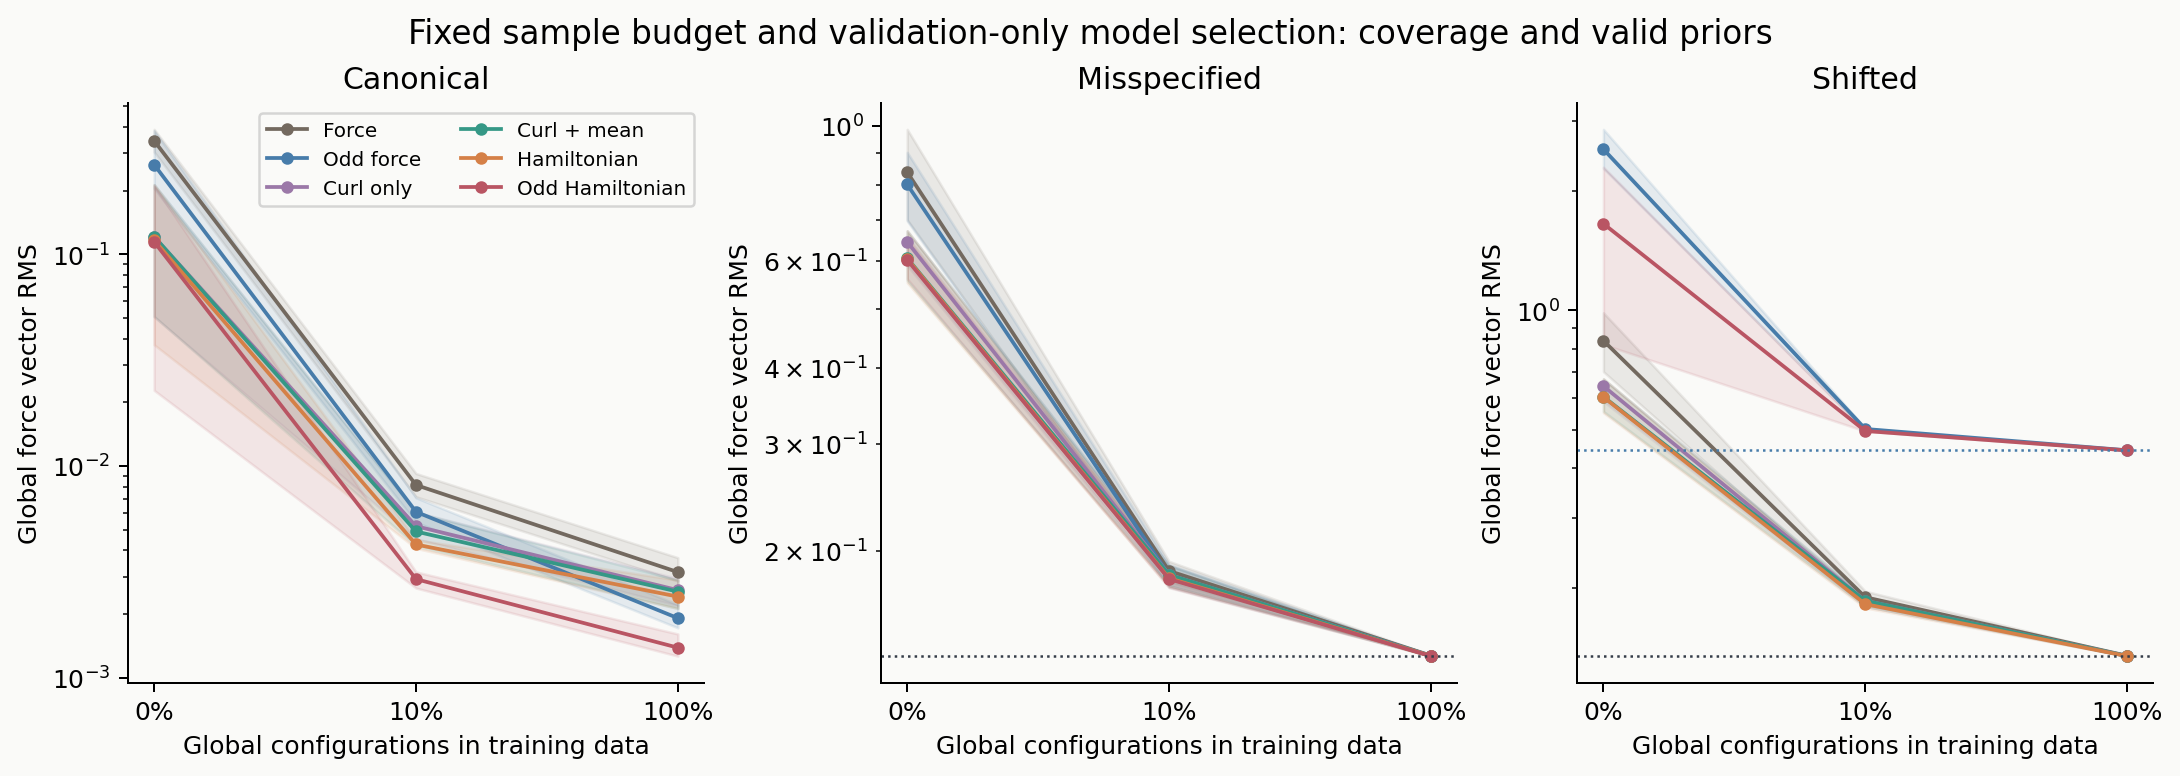
\includegraphics[width=0.95\textwidth,height=\textheight]{../phase6/01_coverage_and_force_error.png}
\caption{Validation-selected coverage and structural priors.}
\end{figure}

\hypertarget{control-and-rl-optimization}{%
\subsection{Control and RL
optimization}\label{control-and-rl-optimization}}

The coupled benchmark includes 220 actual feedback/MPC configurations
and 57 new SAC training runs. SAC uses final checkpoints, 16,000
transitions and 7,492 updates per run, with three world and three policy
seeds in the selected comparisons. All 36 speed-reset interventions are
retained. A reset changes the training distribution and is a limitation,
not an invisible implementation detail.

Hamiltonian MPC mean momentum RMS improves from approximately 0.1258
under local coverage to 0.0304 with mixed coverage and 0.0239 globally.
Unrestricted-force MPC changes from 0.181 to 0.0328 and 0.0240. Under
global unshifted coverage all six force families achieve 100\% strict
success for both tested controller types. The corresponding SAC
comparison remains substantially worse: global momentum RMS is
approximately 0.422 for force, 0.373 for odd force and 0.370 for
Hamiltonian models, against 0.264 for the privileged true-model SAC
reference. The Hamiltonian/odd gap is small relative to the controller
optimization gap.

These results distinguish performance of a fitted model from performance
of a finite-budget optimizer. They do not prove SAC asymptotic failure
or a universal superiority of feedback/MPC. The known-force references
are privileged and are not theoretical lower bounds for every finite
sampled controller.

\begin{figure}
\centering
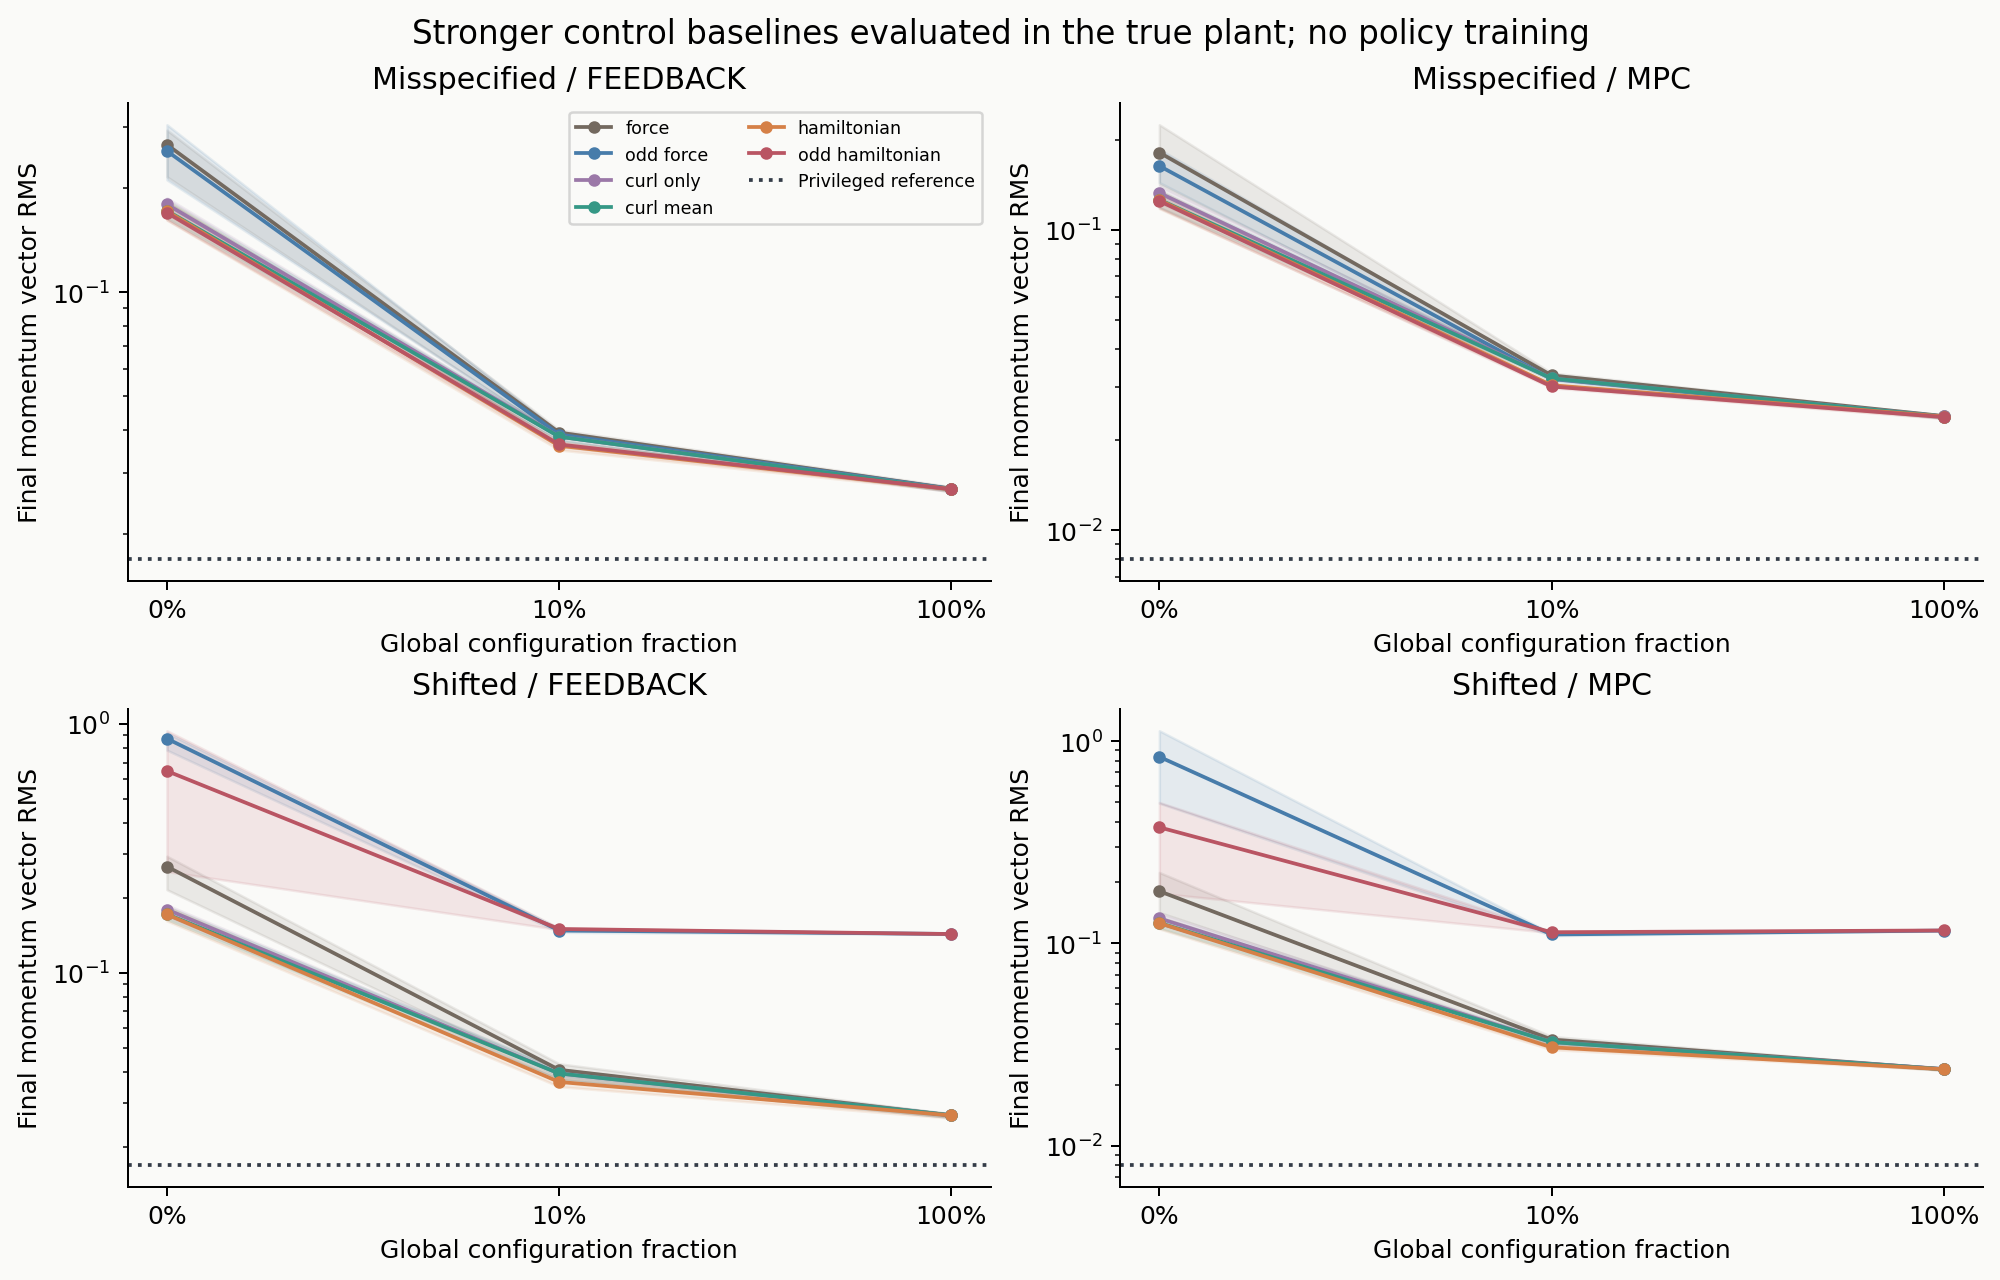
\includegraphics[width=0.95\textwidth,height=\textheight]{../phase6/06_feedback_and_mpc.png}
\caption{True-plant control with feedback and predictive control.}
\end{figure}

\hypertarget{frozen-acquisition-screen}{%
\subsection{Frozen acquisition screen}\label{frozen-acquisition-screen}}

The acquisition study starts with 128 noisy low-energy labels and adds
16, 64 or 256 selected labels from an unlabelled 1,024-configuration
pool. It compares random sampling, pointwise uncertainty, global
A-design, frozen-occupancy A-design and spectral task A-design. Five
paired world seeds, two plant conditions, three force spaces and two
target momenta produce 660 unique fitted models. There are 964 actual
control evaluations; pilot aliases increase reported rows to 1,200 and
are not additional replications. Across paths, 53,760 added-query calls
use 8,001 distinct shared plant/world/pool-index label keys, plus 1,280
unique pilot labels.

The clipped controller runs for 20 time units at held interval 0.05.
Sixty-four fresh uniform configuration phases start exactly at target
momentum. The primary metric is momentum-vector RMS over the final five
time units. This is tracking, not swing-up. The frozen practical gate
requires at least 10\% improvement over the best of four baselines and
at least four of five paired-seed wins in every Hamiltonian B=64 cell,
plus bounded degradation at other budgets.

\begin{longtable}[]{@{}
  >{\raggedright\arraybackslash}p{(\columnwidth - 8\tabcolsep) * \real{0.2000}}
  >{\raggedleft\arraybackslash}p{(\columnwidth - 8\tabcolsep) * \real{0.2000}}
  >{\raggedleft\arraybackslash}p{(\columnwidth - 8\tabcolsep) * \real{0.2000}}
  >{\raggedleft\arraybackslash}p{(\columnwidth - 8\tabcolsep) * \real{0.2000}}
  >{\raggedleft\arraybackslash}p{(\columnwidth - 8\tabcolsep) * \real{0.2000}}@{}}
\toprule\noalign{}
\begin{minipage}[b]{\linewidth}\raggedright
Plant/task
\end{minipage} & \begin{minipage}[b]{\linewidth}\raggedleft
Best baseline RMS
\end{minipage} & \begin{minipage}[b]{\linewidth}\raggedleft
Spectral RMS
\end{minipage} & \begin{minipage}[b]{\linewidth}\raggedleft
Degradation
\end{minipage} & \begin{minipage}[b]{\linewidth}\raggedleft
Seed wins
\end{minipage} \\
\midrule\noalign{}
\endhead
\bottomrule\noalign{}
\endlastfoot
canonical, forward & 0.016906 & 0.017547 & 3.79\% & 2/5 \\
canonical, swapped & 0.015687 & 0.016543 & 5.46\% & 1/5 \\
misspec., forward & 0.034552 & 0.039674 & 14.83\% & 0/5 \\
misspec., swapped & 0.057841 & 0.059162 & 2.28\% & 2/5 \\
\end{longtable}

The candidate fails every primary cell. Random is the best mean baseline
in those cells, established after comparing all four baselines. The gate
is descriptive, not a significance test, and 64 phases do not create 64
independent fitted-world seeds. The new-algorithm route is stopped; no
rescue variants, additional candidate tuning or conditional MPC
confirmations are introduced.

In the misspecified forward task, spectral acquisition reduces posterior
tracking standard deviation from random's 0.00470 to 0.00411, but
increases actual RMS from 0.03455 to 0.03967. The uncertainty criterion
excludes omitted-mode bias. This observed divergence is stronger
evidence against the candidate's practical promise than a favorable
covariance-only plot would be evidence for it.

\begin{figure}
\centering
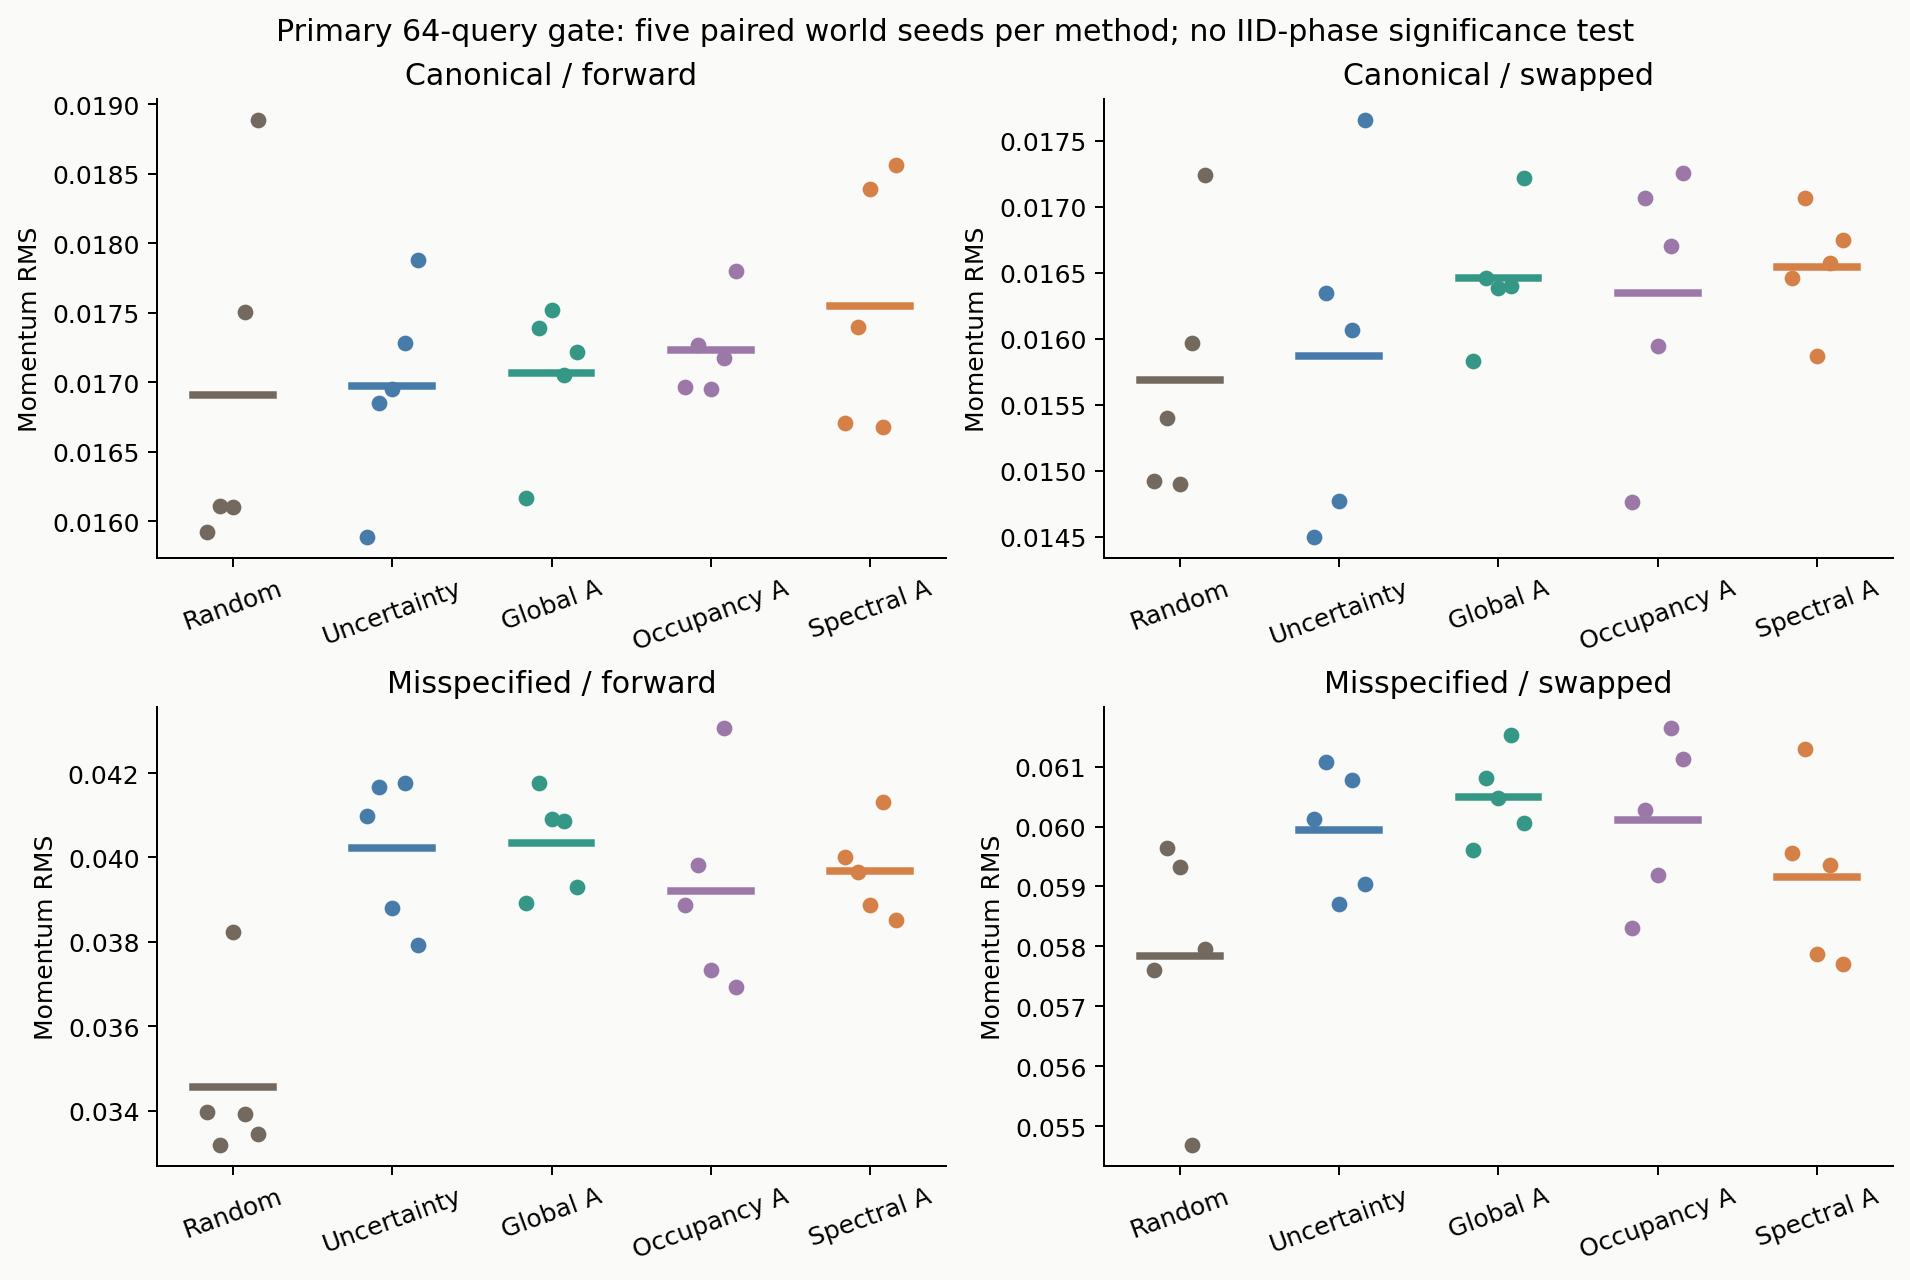
\includegraphics[width=0.95\textwidth,height=\textheight]{../phase7/02_primary_gate_cells.png}
\caption{Frozen acquisition outcomes retain all five world seeds.}
\end{figure}

\hypertarget{independent-validation-and-hold-refinement}{%
\subsection{Independent validation and hold
refinement}\label{independent-validation-and-hold-refinement}}

Coupled Duffing validation produces 45 fits. Mean global force RMS is:

\begin{longtable}[]{@{}lrrr@{}}
\toprule\noalign{}
Coverage & Force (20) & Odd force (12) & Hamiltonian (14) \\
\midrule\noalign{}
\endhead
\bottomrule\noalign{}
\endlastfoot
local & 0.50148 & 0.48487 & 0.40054 \\
10\% global & 0.02146 & 0.01634 & 0.01755 \\
global & 0.00639 & 0.00511 & 0.00507 \\
\end{longtable}

Coverage dominates the between-class difference; odd force slightly
improves on the Hamiltonian mean under mixed coverage. This is
independent-domain support for the coverage interpretation, with
explicit dimension and fixed-ridge limitations. It is not another
acquisition experiment.

The exact-force unsaturated action-hold diagnostic uses 32 shared phases
over ten time units and evaluates the final five. Hold intervals 0.1,
0.05, 0.025 and 0.0125 give momentum RMS 0.035818, 0.017367, 0.008557
and 0.004248. The fitted log-log slope is 1.025. The observed refinement
supports a first-order hold floor in that diagnostic, consistent with
the finite-horizon expansion. It does not quantify every source of error
in the clipped primary test.

\begin{figure}
\centering
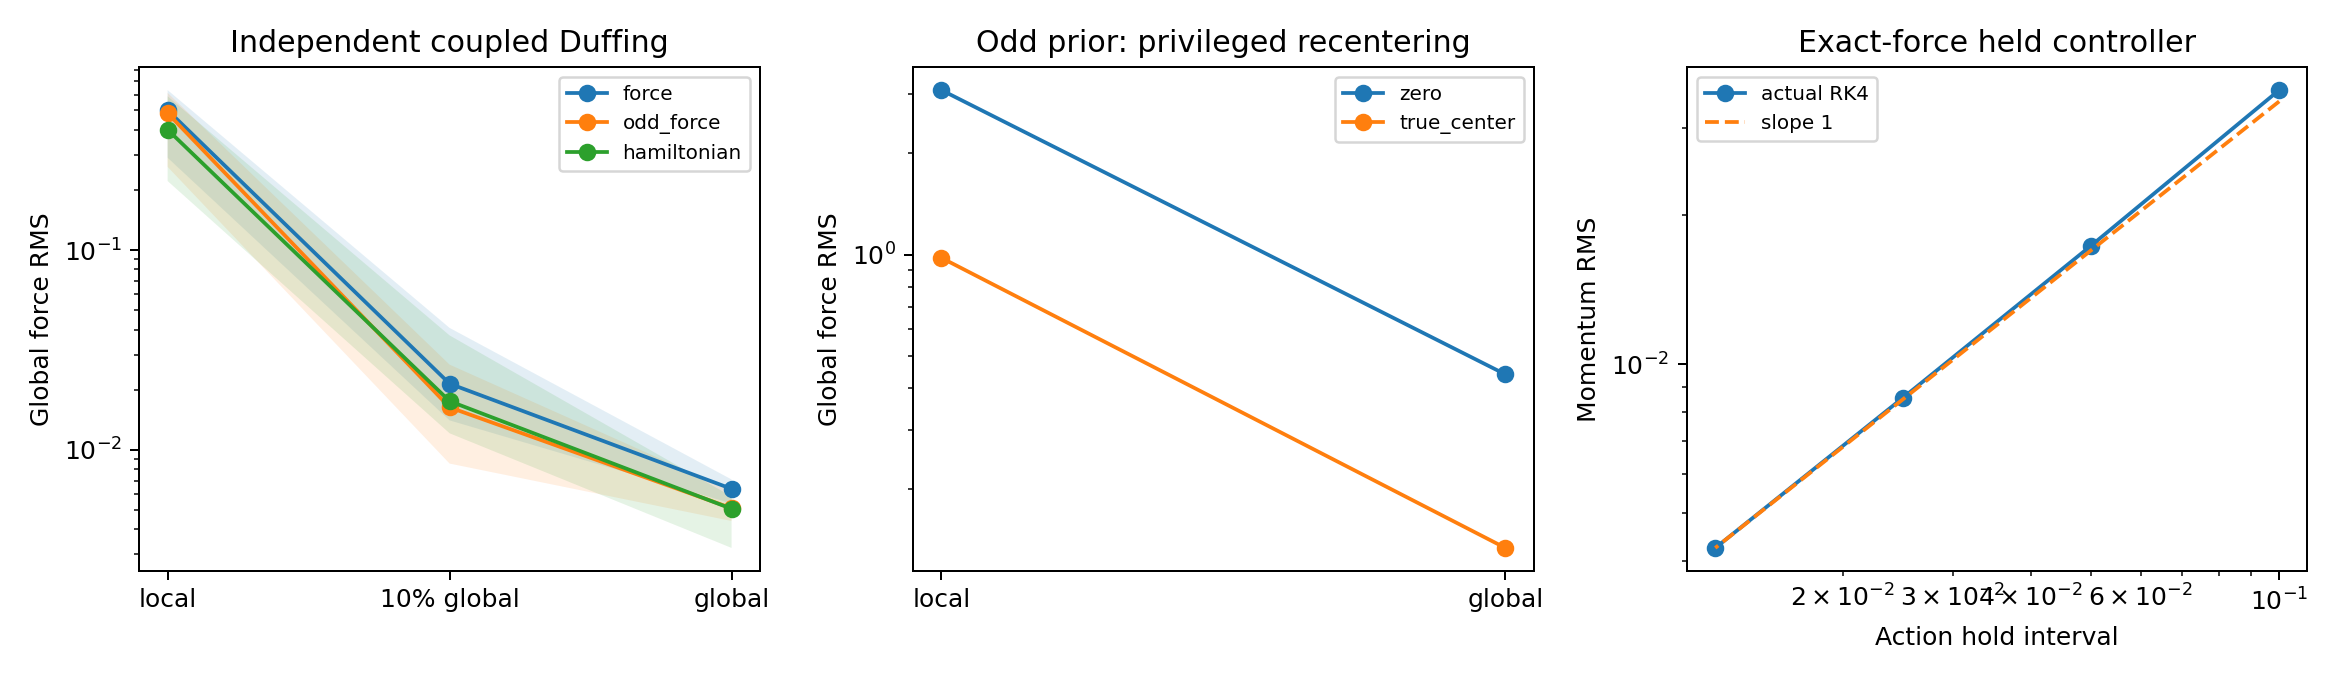
\includegraphics[width=1\textwidth,height=\textheight]{../phase8/final_validation.png}
\caption{Final validation: independent dynamics, privileged recentering
and exact-force action-hold refinement. Shaded Duffing bands show
minimum/maximum across five seeds, not confidence intervals.}
\end{figure}

\hypertarget{simulation-storyboards-and-interpretation}{%
\subsection{Simulation storyboards and
interpretation}\label{simulation-storyboards-and-interpretation}}

Figures below are extracted from the archived numerical animations, not
generated illustrations. The same recorded case is used across every
frame: misspecified periodic plant, Hamiltonian force head, world seed
20 and forward target. The control storyboard additionally fixes
held-out initial phase zero and B=64. Its six panels show one trajectory
under two acquisition rules at three times; they are not six independent
experiments. The rods depict angular coordinates with separate pivots
and an indicated coupling, not the geometry of a serial double pendulum.

\begin{figure}
\centering
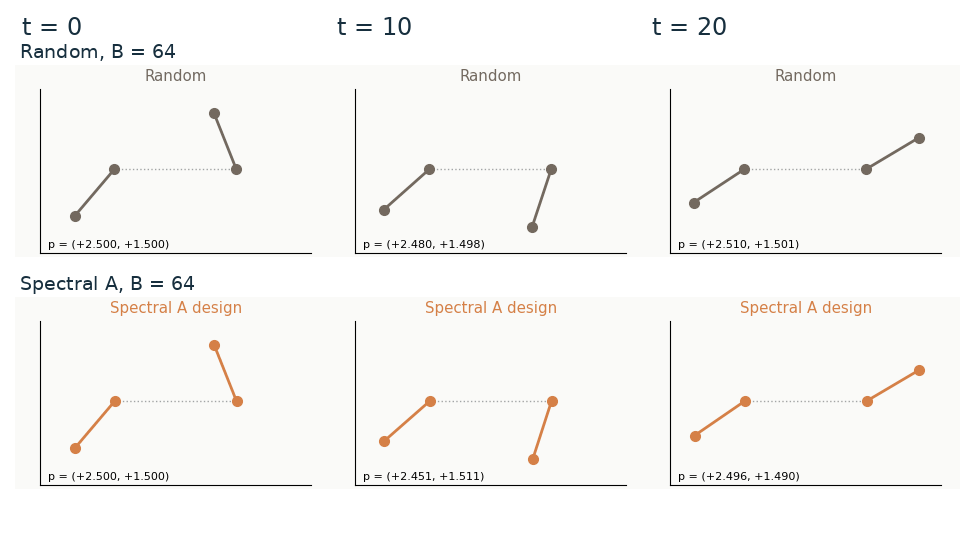
\includegraphics[width=1\textwidth,height=\textheight]{figures/control_animation_filmstrip.png}
\caption{Exact control-animation frames at t=0, 10 and 20. Top: random
acquisition; bottom: spectral A-design, each with 64 added labels and
the same 128-label pilot. Momentum annotations are retained from the
actual RK4 records; full tracking traces remain available in the GIF. A
fixed illustrative trajectory does not determine the aggregate gate.}
\end{figure}

\begin{figure}
\centering
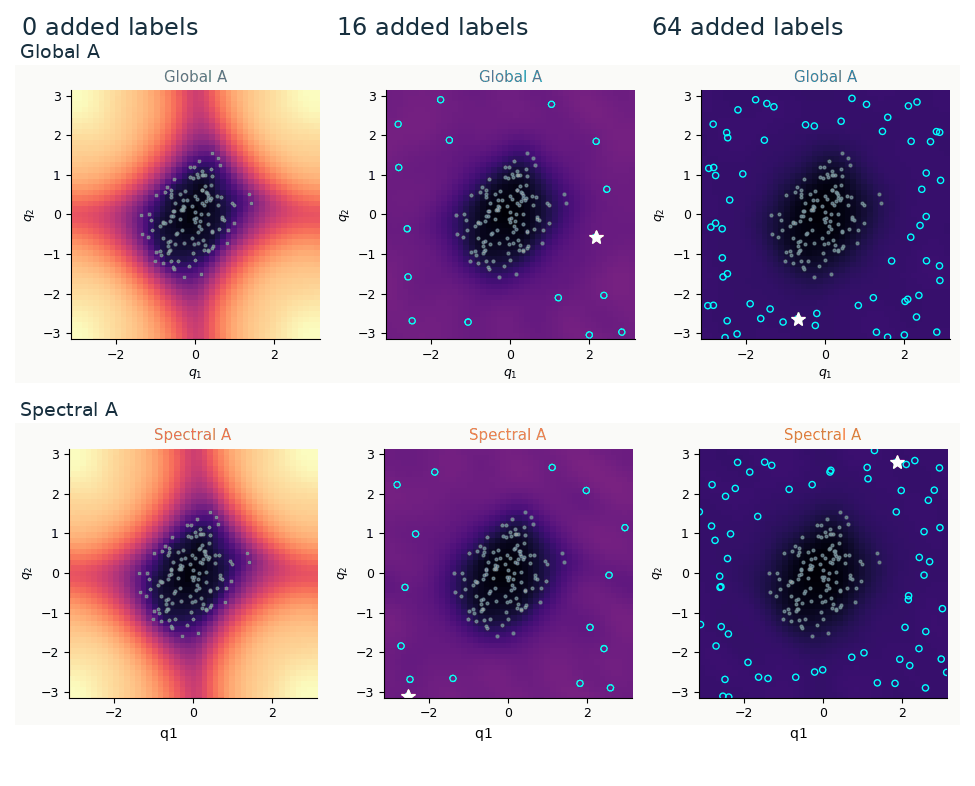
\includegraphics[width=1\textwidth,height=\textheight]{figures/acquisition_animation_filmstrip.png}
\caption{Sequential acquisition storyboard at 0, 16 and 64 added labels.
Grey dots show the shared local pilot; cyan rings are queried
configurations and stars mark the latest query. Top: global A-design;
bottom: spectral A-design. Frames use the identical logarithmic variance
scale shown in the following complete frame. Query count is not physical
time, and posterior variance excludes approximation bias.}
\end{figure}

\begin{figure}
\centering
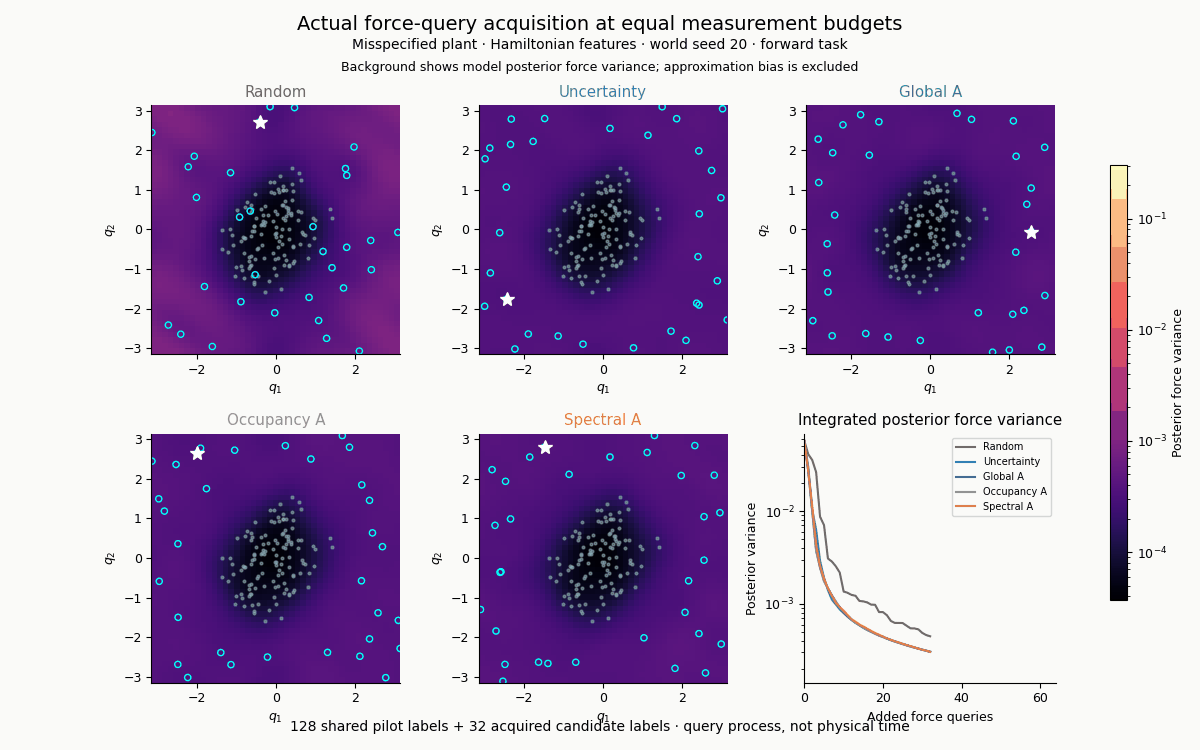
\includegraphics[width=1\textwidth,height=\textheight]{figures/acquisition_frame_32.png}
\caption{Complete acquisition-animation frame at 32 added labels,
retaining the shared logarithmic colorbar, all five methods and the
integrated-variance history. This frame complements the storyboard
without introducing a new numerical evaluation.}
\end{figure}

The corresponding GIFs are
\texttt{phase7/phase7\_control\_comparison.gif} and
\texttt{phase7/phase7\_acquisition.gif}. They play in the repository
README and offline demo; the PDF supplies static multi-frame summaries.
Extraction indices, crop bounds and source hashes are recorded in
\texttt{paper/figures/animation\_stills\_provenance.json}.

\hypertarget{reproducibility-and-verification}{%
\section{Reproducibility and
verification}\label{reproducibility-and-verification}}

The repository contains frozen protocols, raw JSON/CSV records, actual
fitted checkpoints, code, PNG/SVG figures and real trajectory GIFs.
Primary outcomes and posthoc diagnostics are labelled separately.
Earlier failed optimization pilots remain available. No trained
checkpoint is represented as an independently validated universal
policy.

Regression normal equations, independent constrained-force fits,
finite-difference controller gradients, Fourier Parseval identities and
label-query audits check different failure modes. The final Duffing
force/gradient check has maximum error \(9.48\times10^{-11}\); an
independent augmented-QR solution matches a Hamiltonian normal-equation
fit within \(2.10\times10^{-15}\). The largest final normal-equation
residual is \(4.18\times10^{-15}\). Acquisition verification checks
selected labels only, confirms unique indices and protocol fingerprints,
and reproduces the unchanged failed gate.

Full reproduction and a short demonstration are separated. The complete
archive preserves all previous stages; a lightweight GitHub-ready bundle
supplies source, protocols, figures, paper and numerical summaries
without bulky replay/checkpoints. \texttt{ARTIFACT\_INDEX.md} maps every
output to its role. The final release records local validation and does
not claim a remote GitHub publication or a DOI.

\hypertarget{discussion-and-limitations}{%
\section{Discussion and limitations}\label{discussion-and-limitations}}

The strongest supported conclusion is conditional: structural force
restrictions can reduce local estimation variance, but coverage,
coordinate correctness and controller optimization can dominate
practical rankings. Hamiltonian consistency and conserved learned energy
provide useful diagnostics, not identification guarantees. A task-aware
posterior criterion can also be an inadequate proxy for tracking under
approximation bias and sampled control.

There are important limits. Both periodic plants share mechanics; the
translated probe is not a new physical environment. Duffing validation
is estimation-only and uses a correctly specified polynomial potential.
All observations are synthetic, all multidimensional comparators know
mass and ports, and no contact-rich or dissipative robotic plant is
tested. Trainable deep-feature models are not exhaustively compared; the
strongest main results concern exact finite-dimensional force heads.
Five acquisition seeds support a descriptive screen, not broad
statistical generalization. We do not provide full BARL, DYNAMICOED or
published kernel-method replications. The prior literature review is
scoped and cannot certify absolute absence of prior art.

The action-hold analysis deliberately uses an unsaturated reference to
isolate consistency. The main clipped controller can exhibit saturation
and larger-model-error effects. Likewise, posterior covariance excludes
approximation bias, and the fixed-ridge noise calculation excludes
hyperparameter-selection randomness. These distinctions prevent
overinterpreting the analytical identities.

The manuscript's originality lies in its executed, inspectable
comparison and the specific combination of interventions and negative
results. Its mathematics provides a rigorous synthesis of established
tools plus project-specific consistency calculations. A novel general
algorithm, a new general optimal-design theorem and general HNN
superiority are not contributions of this work. Independent review may
judge the empirical contribution appropriate for a workshop,
reproducibility study or technical report rather than a main-conference
methods paper.

\hypertarget{conclusion}{%
\section{Conclusion}\label{conclusion}}

Within the tested settings, Hamiltonian structure helps most when the
force class is valid and observations are local. Broad coverage reduces
that advantage, wrong coordinate-dependent symmetry introduces a
removable floor, and finite-budget RL optimization can obscure improved
world models. The failed acquisition screen and action-hold refinement
show why task-aware uncertainty reduction is insufficient by itself. The
released evidence supports a reproducible conditional account of
Hamiltonian learning for control, with unsuccessful hypotheses retained
as part of the research record.

\clearpage

\hypertarget{references}{%
\section*{References}\label{references}}
\addcontentsline{toc}{section}{References}

\begin{enumerate}
\def\labelenumi{\arabic{enumi}.}
\tightlist
\item
  Greydanus, S., Dzamba, M., and Yosinski, J. (2019). \emph{Hamiltonian
  Neural Networks}. NeurIPS. https://arxiv.org/abs/1906.01563
\item
  Zhong, Y. D., Dey, B., and Chakraborty, A. (2020). \emph{Symplectic
  ODE-Net: Learning Hamiltonian Dynamics with Control}. ICLR.
  https://arxiv.org/abs/1909.12077
\item
  Gruver, N., Finzi, M., Stanton, S., and Wilson, A. G. (2022).
  \emph{Deconstructing the Inductive Biases of Hamiltonian Neural
  Networks}. https://arxiv.org/abs/2202.04836
\item
  Smith, T., and Egeland, O. (2024). \emph{Learning Hamiltonian dynamics
  with reproducing kernel Hilbert spaces and random features}. European
  Journal of Control, 80(B), 101128.
  https://doi.org/10.1016/j.ejcon.2024.101128
\item
  Wagenmaker, A., Simchowitz, M., and Jamieson, K. (2021).
  \emph{Task-Optimal Exploration in Linear Dynamical Systems}. ICML,
  PMLR 139, 10641-10652.
  https://proceedings.mlr.press/v139/wagenmaker21a.html
\item
  Wagenmaker, A., Shi, G., and Jamieson, K. (2023). \emph{Optimal
  Exploration for Model-Based RL in Nonlinear Systems}. NeurIPS.
  https://arxiv.org/abs/2306.09210
\item
  Mehta, V., Paria, B., Schneider, J., Ermon, S., and Neiswanger, W.
  (2022). \emph{An Experimental Design Perspective on Model-Based
  Reinforcement Learning}. ICLR. https://arxiv.org/abs/2112.05244
\item
  Ma, Y. J., Sivakumar, K., Yan, J., Bastani, O., and Jayaraman, D.
  (2023). \emph{Learning Policy-Aware Models for Model-Based
  Reinforcement Learning via Transition Occupancy Matching}. L4DC, PMLR
  211. https://proceedings.mlr.press/v211/ma23a.html
\item
  Pukelsheim, F. (2006). \emph{Optimal Design of Experiments}. SIAM,
  Classics in Applied Mathematics.
  https://epubs.siam.org/doi/book/10.1137/1.9780898719109
\item
  Idais, O., and Schwabe, R. (2021). \emph{Equivariance and Invariance
  for Optimal Designs in Generalized Linear Models Exemplified by a
  Class of Gamma Models}.
  https://link.springer.com/article/10.1007/s42519-021-00221-z
\end{enumerate}

\clearpage

\hypertarget{mathematical-appendix-detailed-derivations}{%
\section*{Mathematical appendix: detailed
derivations}\label{mathematical-appendix-detailed-derivations}}
\addcontentsline{toc}{section}{Mathematical appendix: detailed
derivations}

The following calculations expand the analysis behind the experiments.
All norms on the torus use normalized Haar measure. Statements about
exact continuous dynamics must be separated from statements about the
integrators and held controls. Established identities are not claimed as
new general results.

\hypertarget{a.-canonical-structure-work-balance-and-non-identifiability}{%
\subsection*{A. Canonical structure, work balance and
non-identifiability}\label{a.-canonical-structure-work-balance-and-non-identifiability}}
\addcontentsline{toc}{subsection}{A. Canonical structure, work balance
and non-identifiability}

For \(z=(q,p)\) and \(J=\begin{pmatrix}0&I\\-I&0\end{pmatrix}\), a
controlled Hamiltonian vector field is

\[\dot z=J\nabla H(z)+G u,\qquad G=\begin{pmatrix}0\\I\end{pmatrix}.\]

Since \(J^\top=-J\),

\[\frac{dH}{dt}=\nabla H^\top J\nabla H+\nabla H^\top Gu=p^\top u,\]

\[H(z(T))-H(z(0))=\int_0^T p(t)^\top u(t)\,dt.\]

The experiment therefore measures a work-balance residual, not raw
energy drift during actuation. For a learned force \(\widehat F\) used
without torque, the true-energy derivative is instead

\[\frac{dH(q,\widehat p)}{dt}=\widehat p^\top[\widehat F(q)-F(q)].\]

This term can be nonzero even if the learned Hamiltonian is conserved
exactly. To obtain a conditional quantitative bound, assume
\(\|\widehat F-F\|\le\delta\) and \(\|\widehat p\|\le P\) along the
entire learned trajectory. Then

\[|H(\widehat z(T))-H(\widehat z(0))|\le TP\delta.\]

A small training-domain force error does not establish either bound
along an unseen trajectory.

For explicit non-identifiability, let \(U\) contain all observed
configurations and choose a smooth bump \(b\) supported in an open
region disjoint from \(U\). Define

\[\widetilde V(q)=V(q)+a b(q),\qquad \widetilde F(q)=F(q)-a\nabla b(q).\]

On \(U\), all force labels and all derivatives of the perturbation
vanish. Both vector fields are Hamiltonian, yet outside \(U\) their
difference can be scaled by arbitrary finite \(a\). This construction
assumes an unrestricted smooth potential class; a fixed finite analytic
feature class may instead be identifiable from sufficiently informative
samples. Poor conditioning can nevertheless make finite noisy
extrapolation inaccurate. The smooth bump argument must not be
misrepresented as exact finite-Fourier non-identifiability.

\hypertarget{b.-fourier-curl-periods-and-gradient-force-equivalence}{%
\subsection*{B. Fourier curl, periods and gradient-force
equivalence}\label{b.-fourier-curl-periods-and-gradient-force-equivalence}}
\addcontentsline{toc}{subsection}{B. Fourier curl, periods and
gradient-force equivalence}

Write \(F=c+\sum_k(A_k\cos k^\top q+B_k\sin k^\top q)\) and let
\(k^\perp=(-k_2,k_1)\). Then

\[\partial_{q_1}F_2-\partial_{q_2}F_1
=\sum_k[-(k^\perp\!\cdot A_k)\sin(k^\top q)+(k^\perp\!\cdot B_k)\cos(k^\top q)].\]

Orthogonality implies curl vanishes exactly when \(A_k\) and \(B_k\) are
parallel to \(k\) for every mode. This does not remove \(c\). For each
coordinate-cycle at a fixed transverse coordinate, all nonconstant mode
contributions integrate to zero once the curl-free parallel condition
holds, and the period is

\[\oint_{\gamma_j}F^\top dq=2\pi c_j.\]

Consequently, a finite periodic curl-free force admits a periodic scalar
potential precisely when \(c=0\). If \(A_k=a_k k\) and \(B_k=b_k k\),
one potential satisfying \(F=-\nabla V\) is

\[V(q)=\sum_k[b_k\cos(k^\top q)-a_k\sin(k^\top q)]+C.\]

Thus a Hamiltonian feature head is exactly a constrained-force regressor
under matched objectives. Parameterizing the gradient through a scalar
does not introduce a different statistical estimator if the constrained
subspace, regularizer and labels are the same. The project verifies this
equivalence numerically; differences from unconstrained fitting arise
from the hypothesis class and objective.

Parseval gives

\[\|F\|_2^2=\|c\|^2+\frac12\sum_k(\|A_k\|^2+\|B_k\|^2),\]

\[\|\operatorname{curl}F\|_2^2=\frac12\sum_k[(k^\perp\!\cdot A_k)^2+(k^\perp\!\cdot B_k)^2].\]

These exact population quadratic forms generate the force-norm and curl
penalties; numerical quadrature is unnecessary for those penalties.

\hypertarget{c.-translation-and-the-parity-projection-floor}{%
\subsection*{C. Translation and the parity projection
floor}\label{c.-translation-and-the-parity-projection-floor}}
\addcontentsline{toc}{subsection}{C. Translation and the parity
projection floor}

For \(\theta_k=k^\top s\), translation \(q\mapsto q-s\) rotates
coefficients:

\[\begin{pmatrix}A'_k\\B'_k\end{pmatrix}=
\begin{pmatrix}\cos\theta_k&-\sin\theta_k\\\sin\theta_k&\cos\theta_k\end{pmatrix}
\begin{pmatrix}A_k\\B_k\end{pmatrix}.\]

The rotation acts separately on each force component and preserves
Parseval norm. Parallel coefficients remain parallel, hence Hamiltonian
closure. Sine-only force is not closed under this action.

A true included force mode \(-a k\sin(k^\top(q-s))\) expands as

\[-a k\cos\theta_k\sin(k^\top q)+a k\sin\theta_k\cos(k^\top q).\]

Orthogonal projection onto the zero-centered odd space drops the second
term. Its squared error is \(a^2\|k\|^2\sin^2\theta_k/2\). Summing
included modes and the orthogonal missing frequency yields the
approximation-floor expression in the main text. This is a
population-class minimum. Empirical test estimates may fluctuate below
it, and ridge fits from local data need not approach it.

\hypertarget{d.-exact-fixed-design-bias-variance-decomposition}{%
\subsection*{D. Exact fixed-design bias-variance
decomposition}\label{d.-exact-fixed-design-bias-variance-decomposition}}
\addcontentsline{toc}{subsection}{D. Exact fixed-design bias-variance
decomposition}

Stack componentwise force observations as \(y=X\theta_*+r+\epsilon\),
where \(r\) is a deterministic class-misspecification residual at the
observed locations. Let \(X\) denote the subspace design,
\(D=X^\top X/N\), regularization \(\Lambda\) and \(A=D+\Lambda\). The
fitted coefficients are

\[\widehat\theta=A^{-1}X^\top y/N,\]

\[\overline\theta:=\mathbb E_\epsilon\widehat\theta
=\theta_*-A^{-1}\Lambda\theta_*+A^{-1}X^\top r/N.\]

The first bias term is shrinkage; the second is observed-design aliasing
of omitted dynamics. Orthogonality under a global population measure
does not force \(X^\top r=0\) under a local or finite design.

Let \(R\) be the test-domain coefficient Gram matrix and
\(r_{\rm test}\) the residual of the chosen reference representation.
The total expected test error decomposes as

\[\mathbb E_\epsilon\|\widehat F-F_*\|_{\rm test}^2
=\|F_{\overline\theta}-F_*\|_{\rm test}^2
+\frac{\sigma^2}{N}\operatorname{tr}(RA^{-1}DA^{-1}).\]

The cross term vanishes because the centered estimator has zero mean.
This formula accommodates approximation and design aliasing through the
first term; the posterior covariance \(\sigma^2A^{-1}\) is generally
different from frequentist noise covariance \(\sigma^2A^{-1}DA^{-1}/N\)
in the averaged-loss convention. The two expressions use different
assumptions and precision scaling and must not be interchanged.

For a correctly specified, unregularized full-rank design, \(A=D\) and
variance is \(\sigma^2\operatorname{tr}(RD^{-1})/N\). If \(D\) is close
to \(R\), the leading term is \(\sigma^2 d/N\). With fixed ridge and
population whitening, diagonalizing \(D\) gives the sum in the main
text. With validation-selected ridge, conditioning on that selected
value does not generally restore an unconditional fixed-ridge identity
because selection depends on noise.

\hypertarget{e.-full-periodic-filter-calculation-and-finite-time-correction}{%
\subsection*{E. Full periodic filter calculation and finite-time
correction}\label{e.-full-periodic-filter-calculation-and-finite-time-correction}}
\addcontentsline{toc}{subsection}{E. Full periodic filter calculation
and finite-time correction}

For one vector-valued mode
\(f(t)=A\cos(\theta+\omega t)+B\sin(\theta+\omega t)\), seek
\(e_s=C\cos(\theta+\omega t)+D\sin(\theta+\omega t)\). Matching
coefficients in \(\dot e_s+\kappa e_s=f\) gives

\[\kappa C+\omega D=A,\qquad -\omega C+\kappa D=B,\]

\[C=\frac{\kappa A-\omega B}{\kappa^2+\omega^2},\qquad
D=\frac{\omega A+\kappa B}{\kappa^2+\omega^2}.\]

The cross terms cancel in the response norm:

\[\|C\|^2+\|D\|^2=\frac{\|A\|^2+\|B\|^2}{\kappa^2+\omega^2}.\]

Averaging over uniform torus phase makes different frequency
representatives orthogonal and gives the steady formula. If \(e(0)=0\),
the finite-time solution is

\[e_1(t)=e_s(q_0+p_*t)-e^{-\kappa t}e_s(q_0).\]

This includes the DC contribution \(c(1-e^{-\kappa t})/\kappa\). The
steady expression is therefore not exactly the finite-time
zero-initial-error metric. For each mode, uniform-phase squared error
becomes

\[\frac{\|A_k\|^2+\|B_k\|^2}{2(\kappa^2+\omega_k^2)}
[1+e^{-2\kappa t}-2e^{-\kappa t}\cos(\omega_k t)].\]

The DC squared term is \(\|c\|^2(1-e^{-\kappa t})^2/\kappa^2\). On the
final test window with \(\kappa=2\), this linear-model transient is
negligible, but nonlinear phase drift, saturation and held actions are
not thereby negligible. At resonance \(\omega_k=0\), the formula remains
well-defined; it concerns an ensemble of initial phases, not temporal
decorrelation along one resonant trajectory.

\hypertarget{f.-weighted-design-woodbury-and-invariant-information}{%
\subsection*{F. Weighted design, Woodbury and invariant
information}\label{f.-weighted-design-woodbury-and-invariant-information}}
\addcontentsline{toc}{subsection}{F. Weighted design, Woodbury and
invariant information}

Let \(L=T(T^\top RT)^{-1/2}\) and \(B=\Phi L\). Since
\(\int\Phi^\top\Phi\,dq=R\),

\[\int B(q)^\top B(q)\,dq=L^\top RL=I.\]

The scalar Gaussian prior has precision \(\rho I/\sigma^2\). A
two-component observation adds \(B^\top B/\sigma^2\). Setting
\(A=\rho I+\sum B_i^\top B_i\), Woodbury gives

\[A_{\rm new}^{-1}=A^{-1}-A^{-1}B^\top(I_2+BA^{-1}B^\top)^{-1}BA^{-1}.\]

For a positive-semidefinite task metric \(W\), the exact candidate gain
is

\[g_W(q)=\sigma^2\operatorname{tr}\left[WA^{-1}B^\top(I_2+BA^{-1}B^\top)^{-1}BA^{-1}\right]\ge0.\]

Nonnegativity follows because the covariance reduction is positive
semidefinite. A positive scalar rescaling of \(W\) changes all gains by
that scalar and cannot change the selected maximizer. These gains depend
on locations and covariance, not observed force values, for this fixed
Gaussian linear model.

For completeness, convexity of
\(\Psi(M)=\operatorname{tr}[W(\rho I+nM)^{-1}]\) can be checked along a
symmetric direction \(H\). With \(S=(\rho I+nM)^{-1}\),

\[\frac{d^2}{dt^2}\Psi(M+tH)\bigg|_{t=0}
=2n^2\operatorname{tr}(WSHSHS)\ge0.\]

Indeed \(SHSHS=S^{1/2}(S^{1/2}HS^{1/2})^2S^{1/2}\) is positive
semidefinite. Translation invariance then permits Jensen averaging as in
the main proof. A fixed pilot matrix \(A_0\) that does not commute with
the translations replaces \(\rho I\) and invalidates the invariance
step. Consequently the idealization is not a theorem that the observed
random design must win.

\hypertarget{g.-predictive-control-adjoint-and-sac-objectives}{%
\subsection*{G. Predictive-control adjoint and SAC
objectives}\label{g.-predictive-control-adjoint-and-sac-objectives}}
\addcontentsline{toc}{subsection}{G. Predictive-control adjoint and SAC
objectives}

The MPC model uses kick-drift updates,

\[p_{t+1}=p_t+h[\widehat F(q_t)+u_t],\qquad q_{t+1}=q_t+hp_{t+1}.\]

Writing \(J_t=D\widehat F(q_t)\), the state and input Jacobians are

\[A_t=\begin{pmatrix}I+h^2J_t&hI\\hJ_t&I\end{pmatrix},\qquad
B_t=\begin{pmatrix}h^2I\\hI\end{pmatrix}.\]

For an objective \(C=\sum_{t=0}^{H-1}\ell(z_{t+1},u_t)+\phi(z_H)\),
initialize \(\lambda_H=\nabla\phi(z_H)\). A backward step has

\[g_{u_t}=\partial_u\ell+B_t^\top[\lambda_{t+1}+\nabla_z\ell],\qquad
\lambda_t=A_t^\top[\lambda_{t+1}+\nabla_z\ell].\]

Here \(\ell=h(\|p_{t+1}-p_*\|^2+0.01\|u_t\|^2)\) and
\(\phi=0.5\|p_H-p_*\|^2\). Projected-gradient backtracking guarantees
only nonincrease of this fitted-model objective. It supplies no
true-plant monotonicity or global optimum.

The actual coupled SAC implementation observes

\[o(z)=(\cos q_1,\cos q_2,\sin q_1,\sin q_2,p_1/3,p_2/3),\]

and uses squashed Gaussian torque \(u=2\tanh a\). Its
change-of-variables density is

\[\log\pi(u\mid o)=\sum_j\left[\log\mathcal N(a_j;\mu_j,\sigma_j^2)-\log2-\log(1-\tanh^2a_j)\right],\]

with a small numerical logarithm safeguard in code. Twin critics use
target

\[y=r+\gamma[\min_i\overline Q_i(o',u')-\alpha\log\pi(u'\mid o')],\]

\[\mathcal L_Q=\sum_{i=1}^2\mathbb E(Q_i(o,u)-y)^2,\qquad
\mathcal L_\pi=\mathbb E[\alpha\log\pi(u\mid o)-\min_iQ_i(o,u)].\]

In the coupled implementation, \(\gamma=0.99\), fixed \(\alpha=0.01\),
Adam learning rate \(3\times10^{-4}\) and target interpolation rate
0.005. Reward integrates \(-\|p-p_*\|^2-0.01\|u\|^2\) by substep
trapezoidal quadrature. Replay training uses a continuing-task target
without a terminal multiplier; finite evaluation episodes and recorded
training resets are therefore distinct from a fully specified episodic
Bellman model. These details limit interpretation of finite-budget
policy rankings. The formulas document the implementation; they are
standard SAC objectives, not a new RL method.

\hypertarget{h.-detailed-action-hold-consistency-and-missing-mode-tracking}{%
\subsection*{H. Detailed action-hold consistency and missing-mode
tracking}\label{h.-detailed-action-hold-consistency-and-missing-mode-tracking}}
\addcontentsline{toc}{subsection}{H. Detailed action-hold consistency
and missing-mode tracking}

At a grid state \((q_n,p_n)\) with \(e_n=p_n-p_*\), exact-force
cancellation yields \(\dot p(t_n)=-\kappa e_n\) while the held torque
has zero derivative inside the interval. Hence

\[p_{n+1}=p_n-\kappa h e_n+\frac{h^2}{2}DF(q_n)p_n+O(h^3).\]

A finite-horizon boundedness induction and discrete Gronwall give
\(\sup_n\|e_n\|\le C_T h\). Integrating \(\dot q=p_*+e\) gives
\(q_n=q_0+p_*t_n+O(h)\). Set \(r_n=e_n/h\) and use bounded second
derivatives to replace \(DF(q_n)p_n\):

\[r_{n+1}=r_n+h\left[-\kappa r_n+\frac12DF(q_0+p_*t_n)p_*\right]+O(h^2).\]

Comparing to forward Euler for the response ODE proves
\(r_n=\eta(t_n)+O(h)\). For \(C^2\) periodic forces on a compact torus
and finite \(T\), the derivative assumptions hold; an unbounded
configuration-space system requires a separate bounded-trajectory
neighborhood. Plant integration error must be controlled separately. The
diagnostic fixes RK4 substeps at 0.0025 while varying action-hold
interval, so control sampling is much coarser than integration.

For the periodic missing potential \(\varepsilon[1-\cos(k_*^\top q)]\),
its force amplitude is \(-\varepsilon k_*\sin(k_*^\top q)\). The ideal
first-order squared tracking contribution is

\[\frac{\varepsilon^2\|k_*\|^2}{2[\kappa^2+(k_*^\top p_*)^2]}.\]

With \(k_*=(3,-1)\) and the two targets, \(\omega_*=6\) or 2; at
\(\kappa=2\) and \(\varepsilon=0.06\), RMS contributions are 0.021213
and 0.047434. These are ideal linear response values, not exact
nonlinear tracking lower bounds. The Fourier force approximation floor,
by contrast, is an exact class-level statement.

\end{document}
